\chapter{$^{162}$DY NEGATIVE PARITY STATES}\label{appendix:162Dy_neg}


Appendix \ref{appendix:162Dy_neg} includes a near-final draft of the second of two papers on the lifetimes presented in this dissertation to be submitted to Physical Review C in 2017.

\newpage

% \begin{center}
% \makebox[\textwidth]{
\includegraphics[height=0.95\textheight,page=1]{../162Dy_papers/162Dy_neg202.pdf}\newpage
\includegraphics[height=0.95\textheight,page=2]{../162Dy_papers/162Dy_neg202.pdf}\newpage
\includegraphics[height=0.95\textheight,page=3]{../162Dy_papers/162Dy_neg202.pdf}\newpage
\includegraphics[height=0.95\textheight,page=4]{../162Dy_papers/162Dy_neg202.pdf}\newpage
\includegraphics[height=0.95\textheight,page=5]{../162Dy_papers/162Dy_neg202.pdf}\newpage
\includegraphics[height=0.95\textheight,page=6]{../162Dy_papers/162Dy_neg202.pdf}\newpage
\includegraphics[height=0.95\textheight,page=7]{../162Dy_papers/162Dy_neg202.pdf}\newpage
\includegraphics[height=0.95\textheight,page=8]{../162Dy_papers/162Dy_neg202.pdf}\newpage
\includegraphics[height=0.95\textheight,page=9]{../162Dy_papers/162Dy_neg202.pdf}\newpage
\includegraphics[height=0.95\textheight,page=10]{../162Dy_papers/162Dy_neg202.pdf}\newpage
\includegraphics[height=0.95\textheight,page=11]{../162Dy_papers/162Dy_neg202.pdf}\newpage
\includegraphics[height=0.95\textheight,page=12]{../162Dy_papers/162Dy_neg202.pdf}\newpage
\includegraphics[height=0.95\textheight,page=13]{../162Dy_papers/162Dy_neg202.pdf}\newpage
\includegraphics[height=0.95\textheight,page=14]{../162Dy_papers/162Dy_neg202.pdf}\newpage
\includegraphics[height=0.95\textheight,page=15]{../162Dy_papers/162Dy_neg202.pdf}\newpage
\includegraphics[height=0.95\textheight,page=16]{../162Dy_papers/162Dy_neg202.pdf}\newpage
\includegraphics[height=0.95\textheight,page=17]{../162Dy_papers/162Dy_neg202.pdf}\newpage
\includegraphics[height=0.95\textheight,page=18]{../162Dy_papers/162Dy_neg202.pdf}\newpage
\includegraphics[height=0.95\textheight,page=19]{../162Dy_papers/162Dy_neg202.pdf}

% \end{center}
% 
% 
% 
% \section{Introduction \& Motivation}
% Low-lying excitations in deformed nuclei have been the focus of great experimental and theoretical efforts, with the various vibrational degrees of freedom manifesting in various forms in well-deformed nuclei. The earliest geometric considerations place the dynamic octupole vibration as a fragmented quartet of states with K$^\pi$ projections 0$^-$, 1$^-$, 2$^-$, and 3$^-$ \cite{BohrMott_text}.
% Strong octupole shape correlations have been experimentally observed in spherical/transitional nuclei (and in extremely neutron rich $^{144}$Ba) \cite{Bucher_Octupole144Ba_2016,Garrett_2009_negShapeCoex} by the observation of strong B(E3) transitions to the ground state, and corresponds to the early microscopic formulation by Neergard \cite{NEERGARD197033}. In well-deformed nuclei (where the ratio to the ground state 4$^+$ to 2$^+$ energies approaches and exceeds 3), the splitting and fragmentation of the octupole modes has presented distinct challenges, with the ordering inversion of negative parity bands with increasing A, and a preferential decay pattern to the ground state of the K$^\pi$=0$^-$ band over the K$^\pi$=1$^-$ band \cite{Casten_text}. This degree of K-forbidedness is extended in the quartet of negative parity states, with experimentally measured hindrances of transition probabilities for $\Delta$K$>$1 \cite{Garrett_2009_negShapeCoex}, but the full systematic evolution of any octupole strength across the range of fragmented negative parity states is yet to be established. To complicate matters further, the coupling of octupole and quadrupole vibrations has been observed in strong K$^\pi$=2$^-\rightarrow$K$^\pi$=2$^+_\gamma$ transitions (in the form of a 2$^+\otimes$3$^-$ phonon coupling) in several nearby cases \cite{Pascu_octupole_2015,Maser_E1s_168Er}, which mirrors and expands upon the feasibility of multi-phonon quadrupole states in deformed nuclei \cite{Aprahamian2004, WuAprahamian_multiphonon_1994}. However, this decay pattern is new and distinctly contrasted with the historical notion of octupole collectivity being built on top of the ground state. The existence of strong E1 transitions in this interband case is not without its own set of challenges, in that modern theoretical descriptions do not correctly predict this behavior (globally or locally), and that this behavior is \textit{sui generis} in the deformed rare-earth region of nuclei, and works stress that this should not be applied systematically across the region, even with the observed cases of nearby and nearly spherical/transitional $^{152}$Sm and $^{150}$Nd \cite{Chakraborty_negparity2012}. 
% % Due to the general lack of lifetime data available for the low-lying negative parity states in deformed nuclei, the evolution of the electric dipole structure of these states is cloudy in practice. 
% Even with recent advancements of the \textit{spdf} IBM, octupole correlations remain cloudy in the rare-earth region, implying some extranneous interpretation or origin of octupole and electric dipole strength with regards to the inclusion of the \textit{p} and \textit{f} bosons \cite{Aprahamian200642}.
% 
% \begin{figure}[h] 
% \begin{center}
% 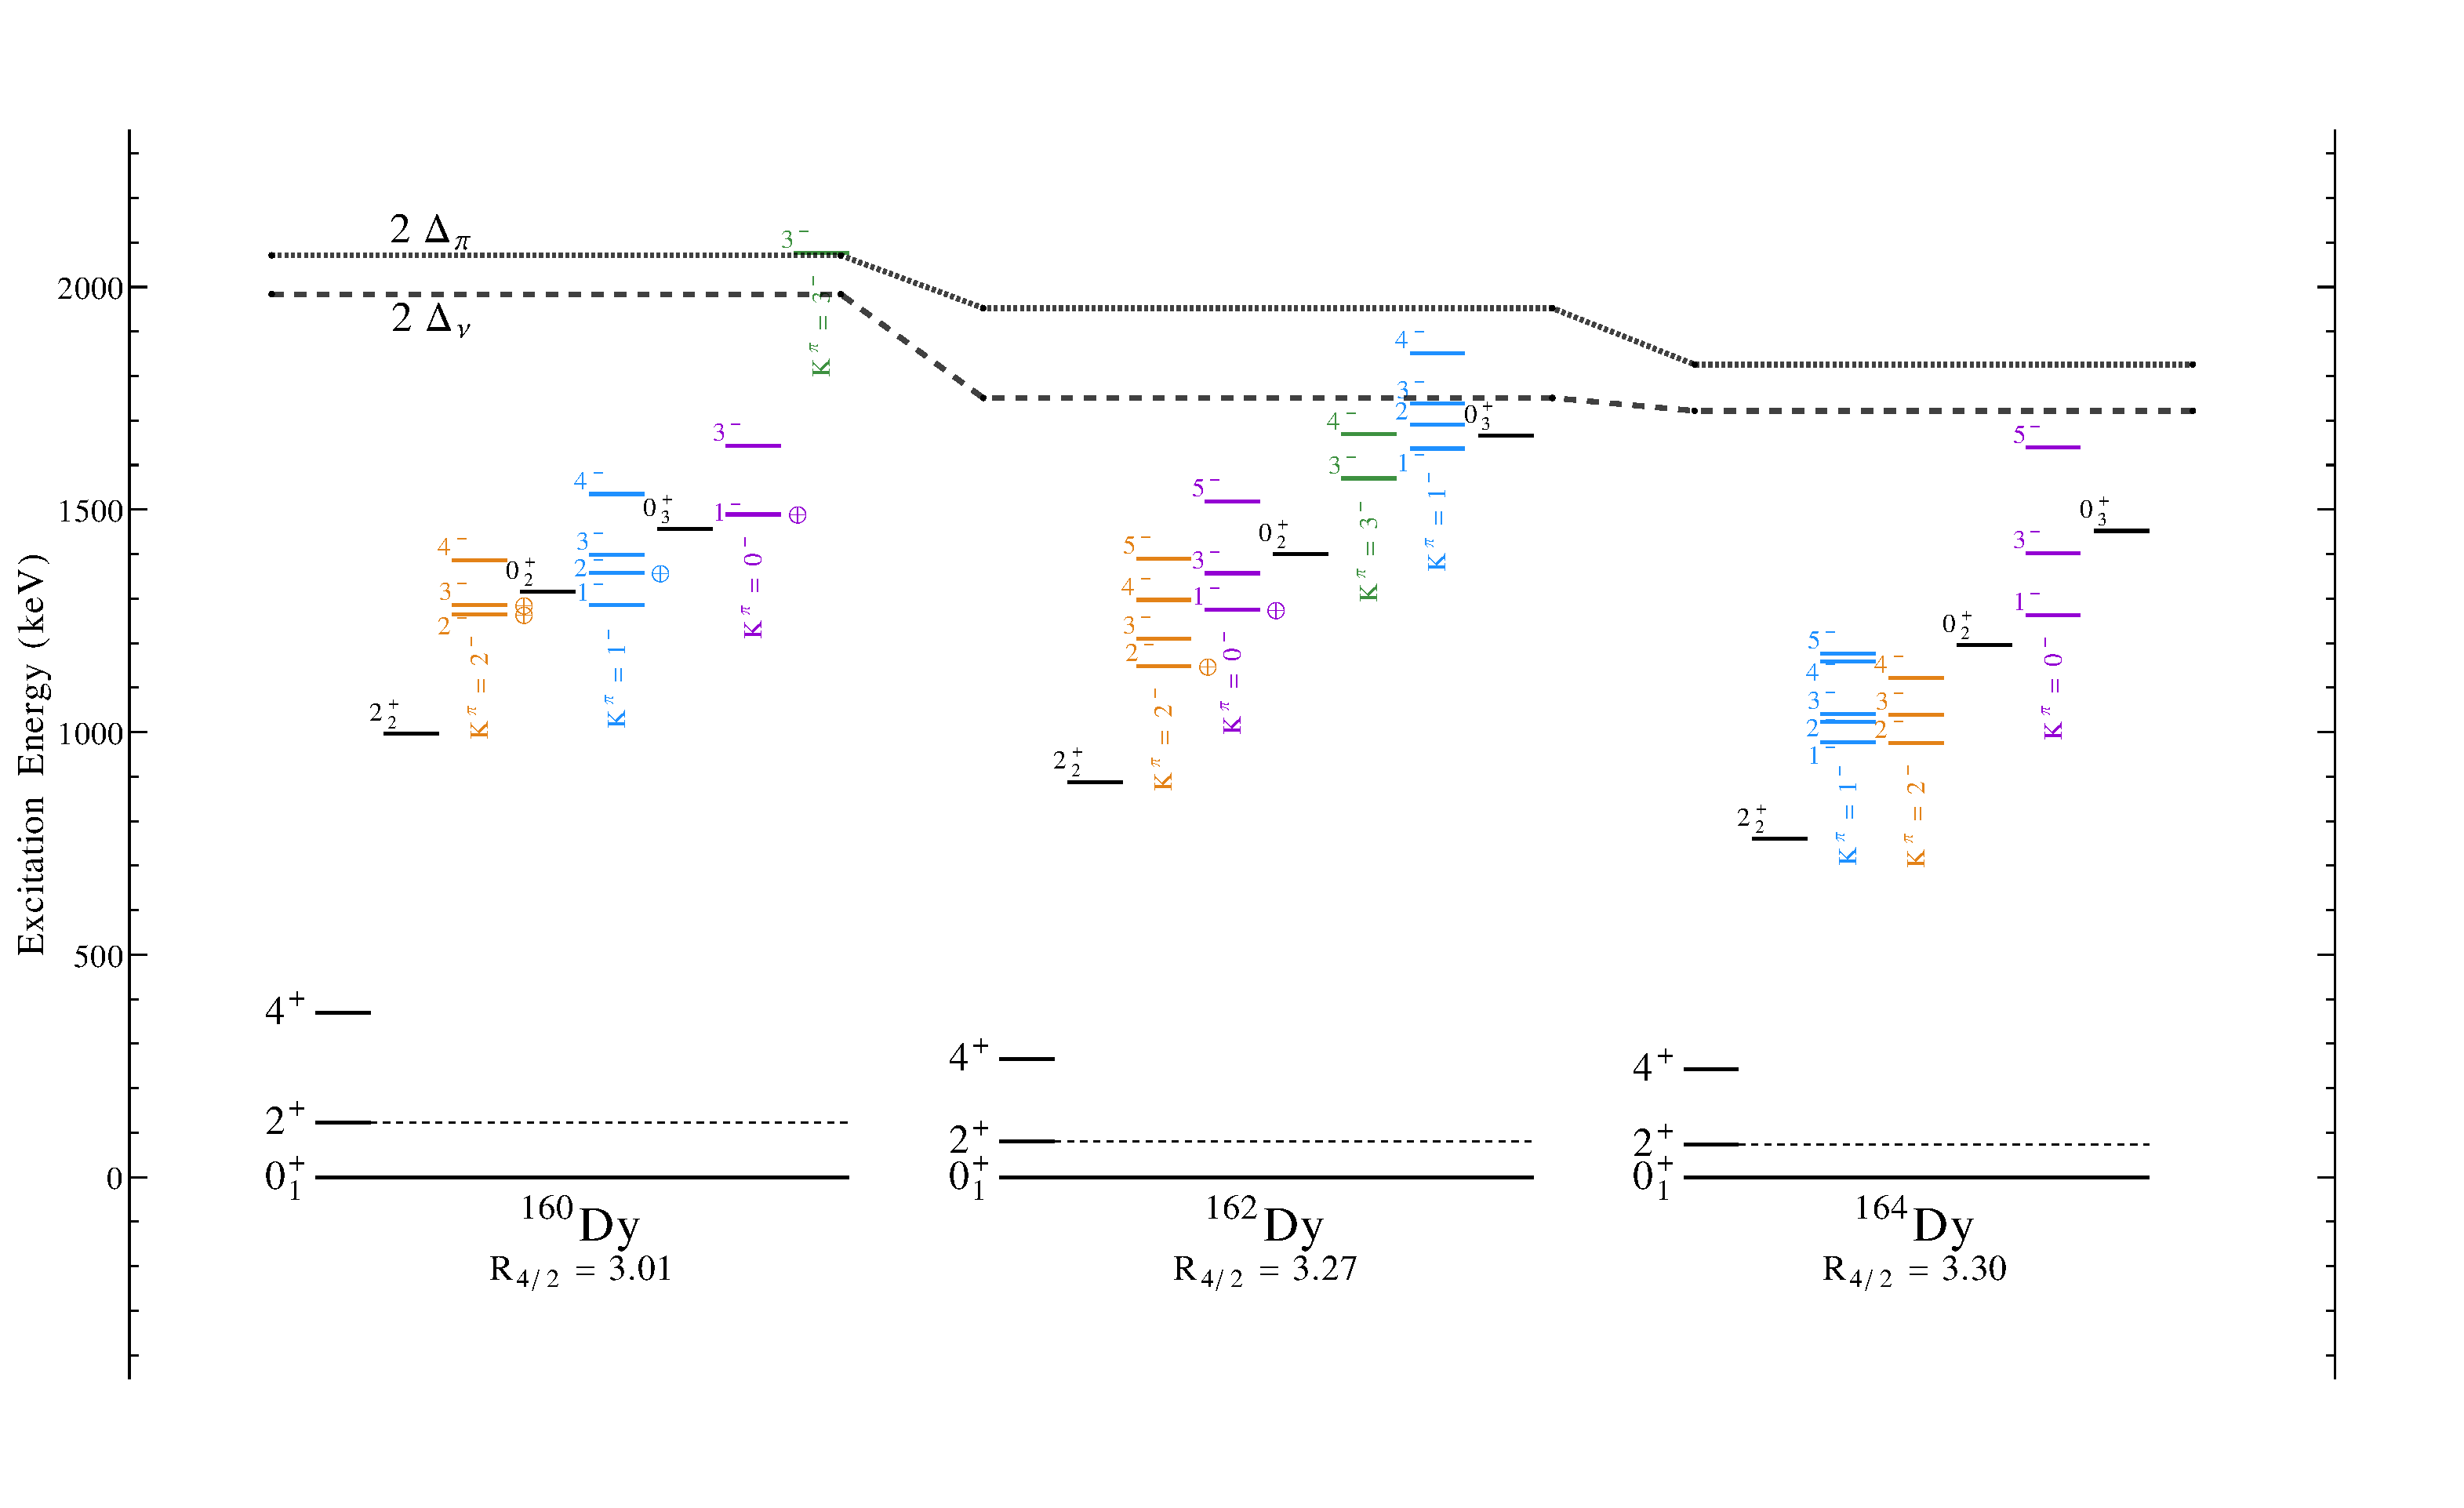
\includegraphics[width=0.98\textwidth]{../Dissertation_Casarella/SciDraw_DySystematics_Octupole.pdf}
% \caption{Negative parity bands below the proton and neutron pairing gaps (2$\Delta_\pi$ \& 2$\Delta_\nu$, respectively) in $^{160-164}$Dy nuclei (color online). Levels with an associated literature lifetime are marked with a ``$\bigoplus$" on the right of each level. (We dispute the two literature lifetime values for $^{162}$Dy in this work.) \label{fig:app_Dy_Octupole_systematics}}
% \end{center}
% \end{figure}
% 
% In $\gamma$-singles experiments with modest detection efficiency, higher-order multipolarity radiation is exponentially diminishing in intensity, making observation of the direct electric octupole (E3) radiation difficult. Although the direct correlation of octupole strength is not governed by E1 transitions directly, the E1 transition strengths are an indication of reflection-asymmetry, making it useful to discern the standard $\lambda$=3 dynamic deformation in form. Measurement of absolute strong E1 transitions are not the `smoking gun' of octupole deformation, but are still indicative and critical in the determination of any single and/or double phonon octupole characteristics in deformed nuclei, as other modes of collective excitations may arise via the electric dipole strengths between nuclear states \cite{Spiecker_E1strength}. Calculation of these reduced transition probabilities is achieved via the measurement of nuclear lifetimes, branching ratios, and $\gamma$-ray energies.
% 
% Energetics for the lowest-lying negative parity states in Dysprosium nuclei can be seen in Figure \ref{fig:app_Dy_Octupole_systematics}, where the energy inversion and variation of the lowest-lying negative K$^\pi$ bands can immediately be seen. At the risk of redundancy by mirroring the assertions made by the numerous preceeding works with regards to quadrupole excitations in deformed nuclei, consistent measurement of nuclear lifetimes will allow the full elucidation of the negative parity states in the rare earth region of nuclei (whether they are quasiparticle excitations, stable octupole deformations, octupole degrees of freedom on top of quadrupole modes, or something completely different). No rare-earth nucleus contains lifetime information for all four negative parity bands (0$^-$, 1$^-$, 2$^-$, \& 3$^-$) surmised to be a part of the octupole vibration, and $^{162}$Dy is no exception to this rule. Furthermore, we can motivate the measurement of lifetimes in $^{162}$Dy by the clear lack of lifetime information for the vast majority of negative parity states in Dysprosium nuclei (6 literature lifetimes exist in the $^{160-164}$Dy chain - seen in Figure \ref{fig:app_Dy_Octupole_systematics}) and the seemingly enigmatic nature and systematics of octupole correlations in the rare-earth region.
% \section{Experiment}
% Lifetimes of excited states were measured with the Doppler Shift Attenuation Method via Inelastic Neutron Scattering (DSAM-INS), a technique that exploits the fact that any emitted radiation from a recoiling nucleus will be energy shifted with respect to the laboratory angle of observation. De-exciting $\gamma$-rays will be Doppler shifted linearly as a function of $\cos$($\theta_{lab}$), the unshifted $\gamma$-ray energy \textit{E}$_{\gamma,o}$, the recoil velocity of the decaying nucleus $\beta$, and a lifetime-dependent attenuation factor \textit{F}($\tau$), all shown in Equation \ref{eq:F(tau)}. 
% \begin{equation} \label{eq:F(tau)}
% E_{\gamma}(\theta_{lab})=E_{\gamma,o}[1+\beta F(\tau)\cos(\theta_{lab})]
% \end{equation}
% 
% Population of excited states (and subsequent nuclear recoil) is achieved with a $^{162}$Dy(n,n$^\prime\gamma$) reaction at the University of Kentucky Accelerator Laboratory (UKAL). Pulsed, bunched protons are accelerated by the 7~MV Van De Graaff accelerator on site, where they impinge on a pressurized $^3$H gas cell at the end of the beamline to create neutrons according to the $^3$H(p,n) reaction. Neutrons then scatter inelastically off a polyethelene vial containing enriched $^{162}$Dy oxide powder. De-exciting $\gamma$-rays are observed in $\gamma$-singles mode by the single Ortec HPGe detector equipped with both passive and active shielding \cite{Garrett_DSAM_INS2000, Belgya_DSAM1996}. A schematic drawing of the experimental setup at UKAL is shown in Figure \ref{fig:app_ExpSetup}. 
% 
% \begin{figure}[h] 
% \begin{center}
% 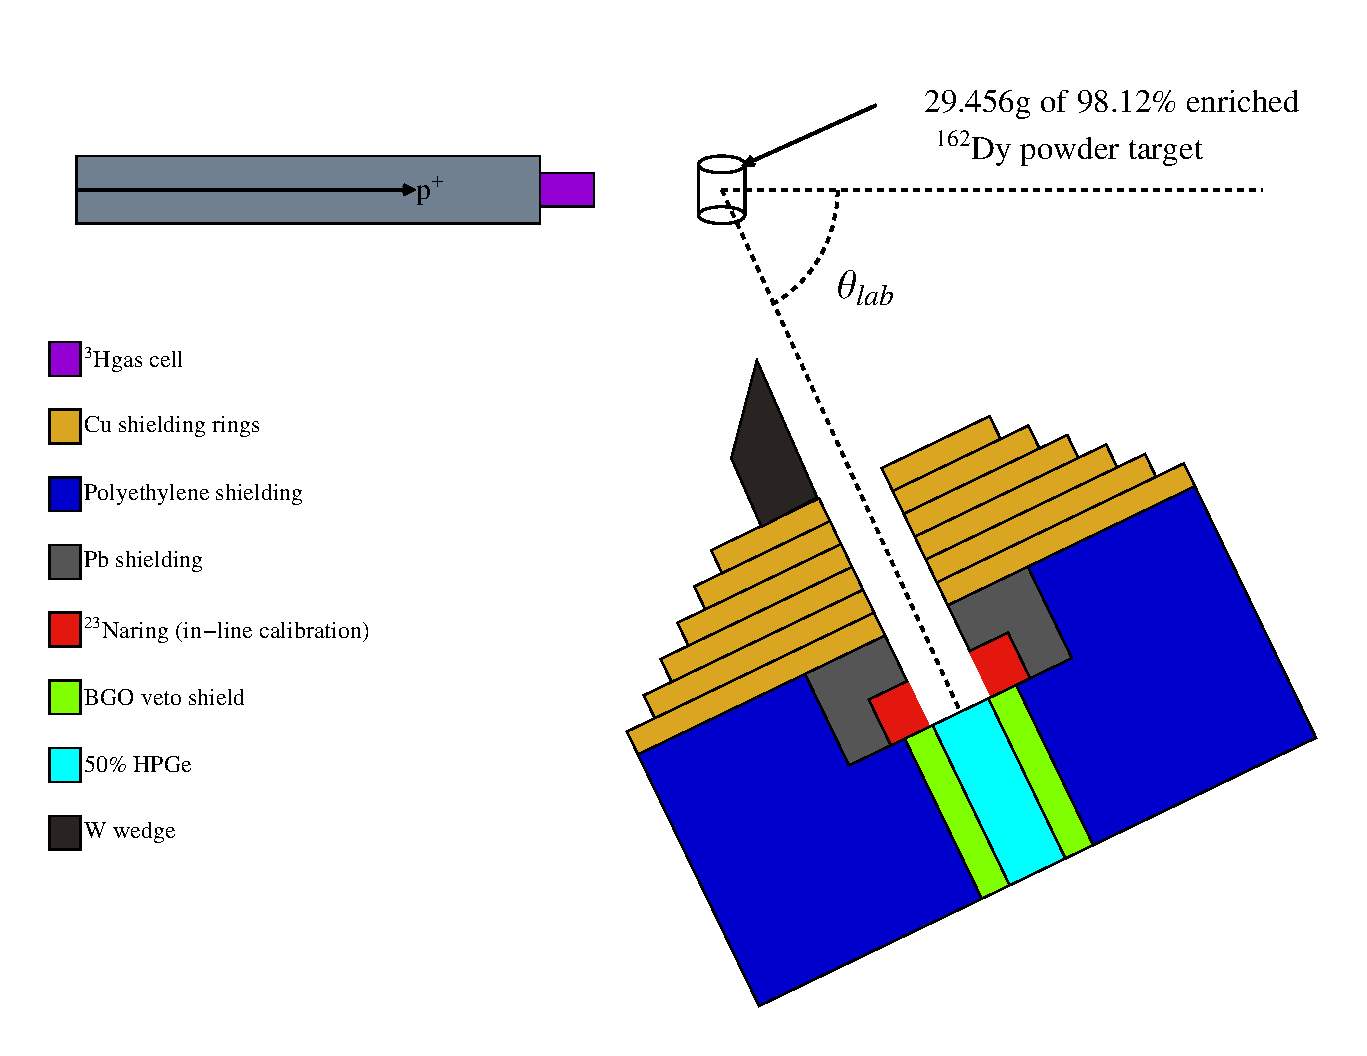
\includegraphics[width=0.95\textwidth]{../Dissertation_Casarella/SciDraw_ExpSetup_Dy.pdf}
% \caption{Not-to-scale cartoon of experimental setup (color online) at UKAL for $\gamma$-singles measurements (Made in M. Caprio's SciDraw software for Mathematica [REF])}
% \label{fig:app_ExpSetup}
% \end{center}
% \end{figure}
% 
% Two experiments are performed with this setup, excitation function and angular distribution measurements; the excitation functions serve to confirm population thresholds of $\gamma$-rays to confidently place them in the level scheme. The gross population rate of states as a function of neutron energy can also be inferred from the excitation functions, and act as a guide in choosing optimal neutron energies to perform angular distribution measurements. Excitation function measurements also aid in the selection of appropriate bombarding neutron energies, as any contaminants or $\gamma$ rays of a similar energy ca The inelastic scattering reaction used to populate states in $^{162}$Dy serves multiple beneficial experimental facets: the use of neutrons as a probe forgoes any need to overcome the Coulomb barrier of the nucleus, is generally non-selective on the type of excitations populated (single particle, collective excitations, etc are all populated), and will realistically only populate J$^\pi\leq$5$^\pm$ excitations. 
% 
% The $\sim$50\% HPGe detector sits 125~cm away from the suspended sample of Dy powder, and can be moved on a circular track to observe $\gamma$-rays at various lab angles to populate the angular distribution measurements needed to measure the lifetimes of states. 
% 
% Angular distributions were collected at angles between 40 and 150 degrees with respect to the beam direction over the course of the experimental campaign. Measurement of the angular distributions offers several distinct assets for nuclear structure studies; absolute intensities of $\gamma$-rays, inferred multipolarities (and multipole mixing fractions) of $\gamma$-rays, and most importantly, the extraction of \textit{F}($\tau$) are all achieved in the angular distribution experiments at UKAL. Confirmation of dipole, E1 radiation (shown in Figure \ref{fig:app_multipole_diff}) can be made by examination of the relative sign/magnitude of the a$_2$ and a$_4$ coefficients in Equation \ref{eq:angdistW} (a$_2$<0 for E1/M1 radiation); absolute intensities of $\gamma$-rays can also be extracted from the A$_0$ parameter. 
% 
% 
% \begin{figure}[h] 
% \begin{center}
% 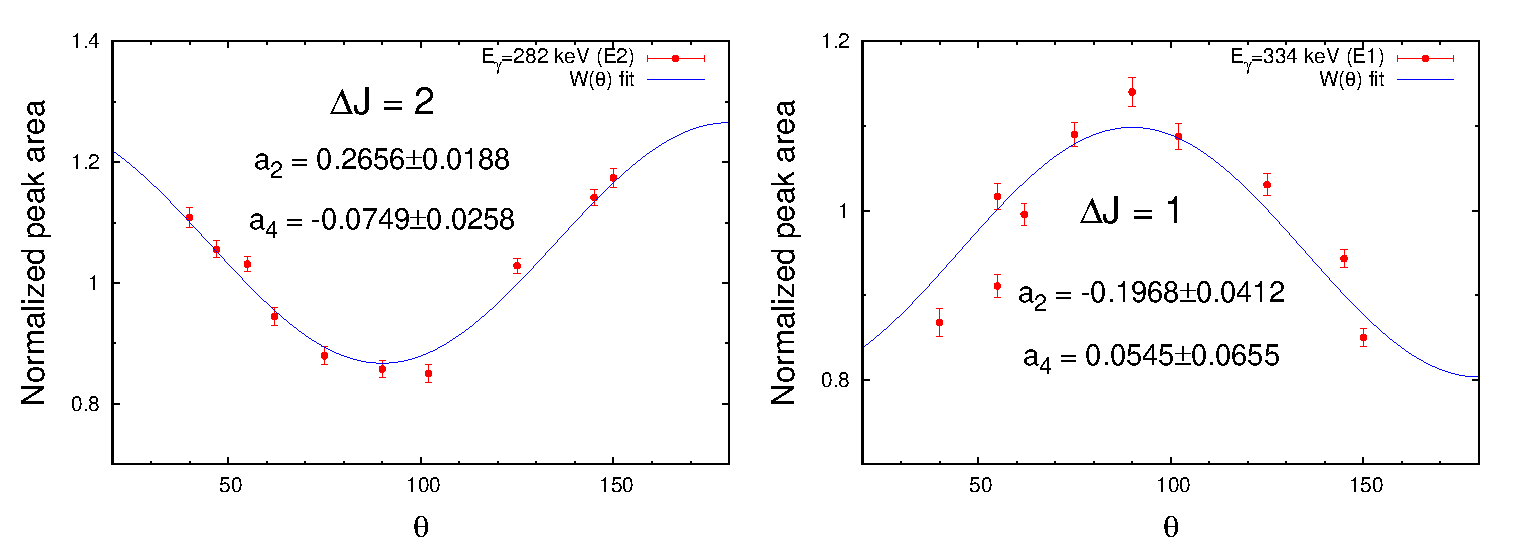
\includegraphics[width=0.95\textwidth]{../Dissertation_Casarella/multipole_diff.eps}
% \caption{Angular distributions from two multipolarity $\gamma$-rays, highlighting the distinct radiation pattern for varying multipolarities. \label{fig:app_multipole_diff}}
% \end{center}
% \end{figure}
% 
% 
% \begin{equation} \label{eq:angdistW}
% W(\theta) \approx \text{A}_0[1+\text{a}_2\text{P}_2(\cos\theta_{lab})+\text{a}_4\text{P}_4(\cos\theta_{lab})]
% \end{equation}
% 
% To extract the lifetime of a state from the angular distribution, energy shifts of $\gamma$-rays are observed as a function of angle, and are fit linearly according to Equation \ref{eq:F(tau)}, where the slope is \textit{F}($\tau$). The experimental \textit{F}($\tau$) factors for a particular $\gamma$-ray are compared with theoretical calculations of this lifetime-dependent attenuation according to the Winterbon formalism outlined in \cite{WINTERBON_1975}. The sensitivity and applicability of DSAM-INS lifetimes is dependent on both the nuclear and electronic stopping powers of the target, which places an effective range of $\sim$10-2000~fs on the lifetimes measurable with this method. Lifetimes outside of this range will exhibit very small energy-shifts over the range of angles used in the measurement, and will be reported as lower limits for the lifetime.
% 
% Spectra from angular distributions are TOF gated for active background subtraction, have a 5$^{th}$-order polynomial ADC nonlinearity applied, and are efficiency calibrated using an offline $^{226}$Ra source. 
% \section{Results \& Discussion}
% We have measured a wealth of lifetimes for J$^\pi\leq$5$^\pm$ states in $^{162}$Dy, shown in Figure \ref{fig:app_162Dy_viz_lifetimes}. Of these 68 lifetimes, we have observed decays from this lowest-lying quartet of negative parity states (Figure \ref{fig:app_162Dy_LLoct}), however, the measured F($\tau$) values for the 1$^-$ and 3$^-$ bands are either conistent with zero within 1$\sigma$ or outright negative in value. This acts as a flag to tell us that these 1$^-$ and 3$^-$ band lifetimes are not reliable; as such, they are not discussed in this work and need refinement with other lifetime measurement techniques. To further indicate unreliable lifetime measurement of the 1$^-$ and 3$^-$ bands, comparison of the calculated transition probabilities to the Alaga rules yield a vast discrepancy. This disagreement with Alaga \textit{may} indicate that these bands are indeed not part of the octupole vibration coupled to the rotational ground state, but instead could be the product of mixing (another 3$^-$ band appears at 1766~keV).
% 
% \begin{figure}[h]
% \begin{center}
% 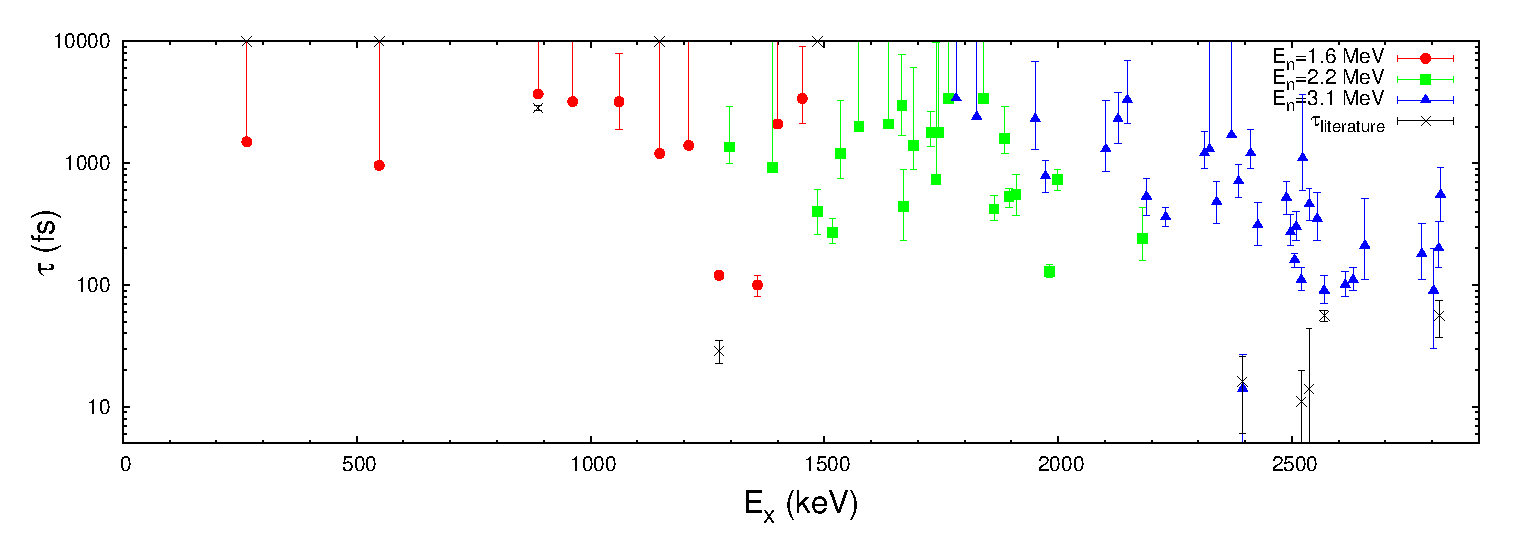
\includegraphics[width=0.999\textwidth]{../Dissertation_Casarella/162Dy_viz_lifetimes.eps}
% \caption{All measured lifetimes in $^{162}$Dy (in femtoseconds) plotted as a function of excitation energy in keV. Data points in red are extracted from the E$_n$=1.6~MeV angular distributions, points in green correspond to lifetimes extracted from the 2.2~MeV angular distributions, and blue points are lifetimes from the 3.1~MeV dataset. (color online) \label{fig:app_162Dy_viz_lifetimes}}
% \end{center}
% \end{figure}
% 
% \begin{figure}[h] 
% \begin{center}
% 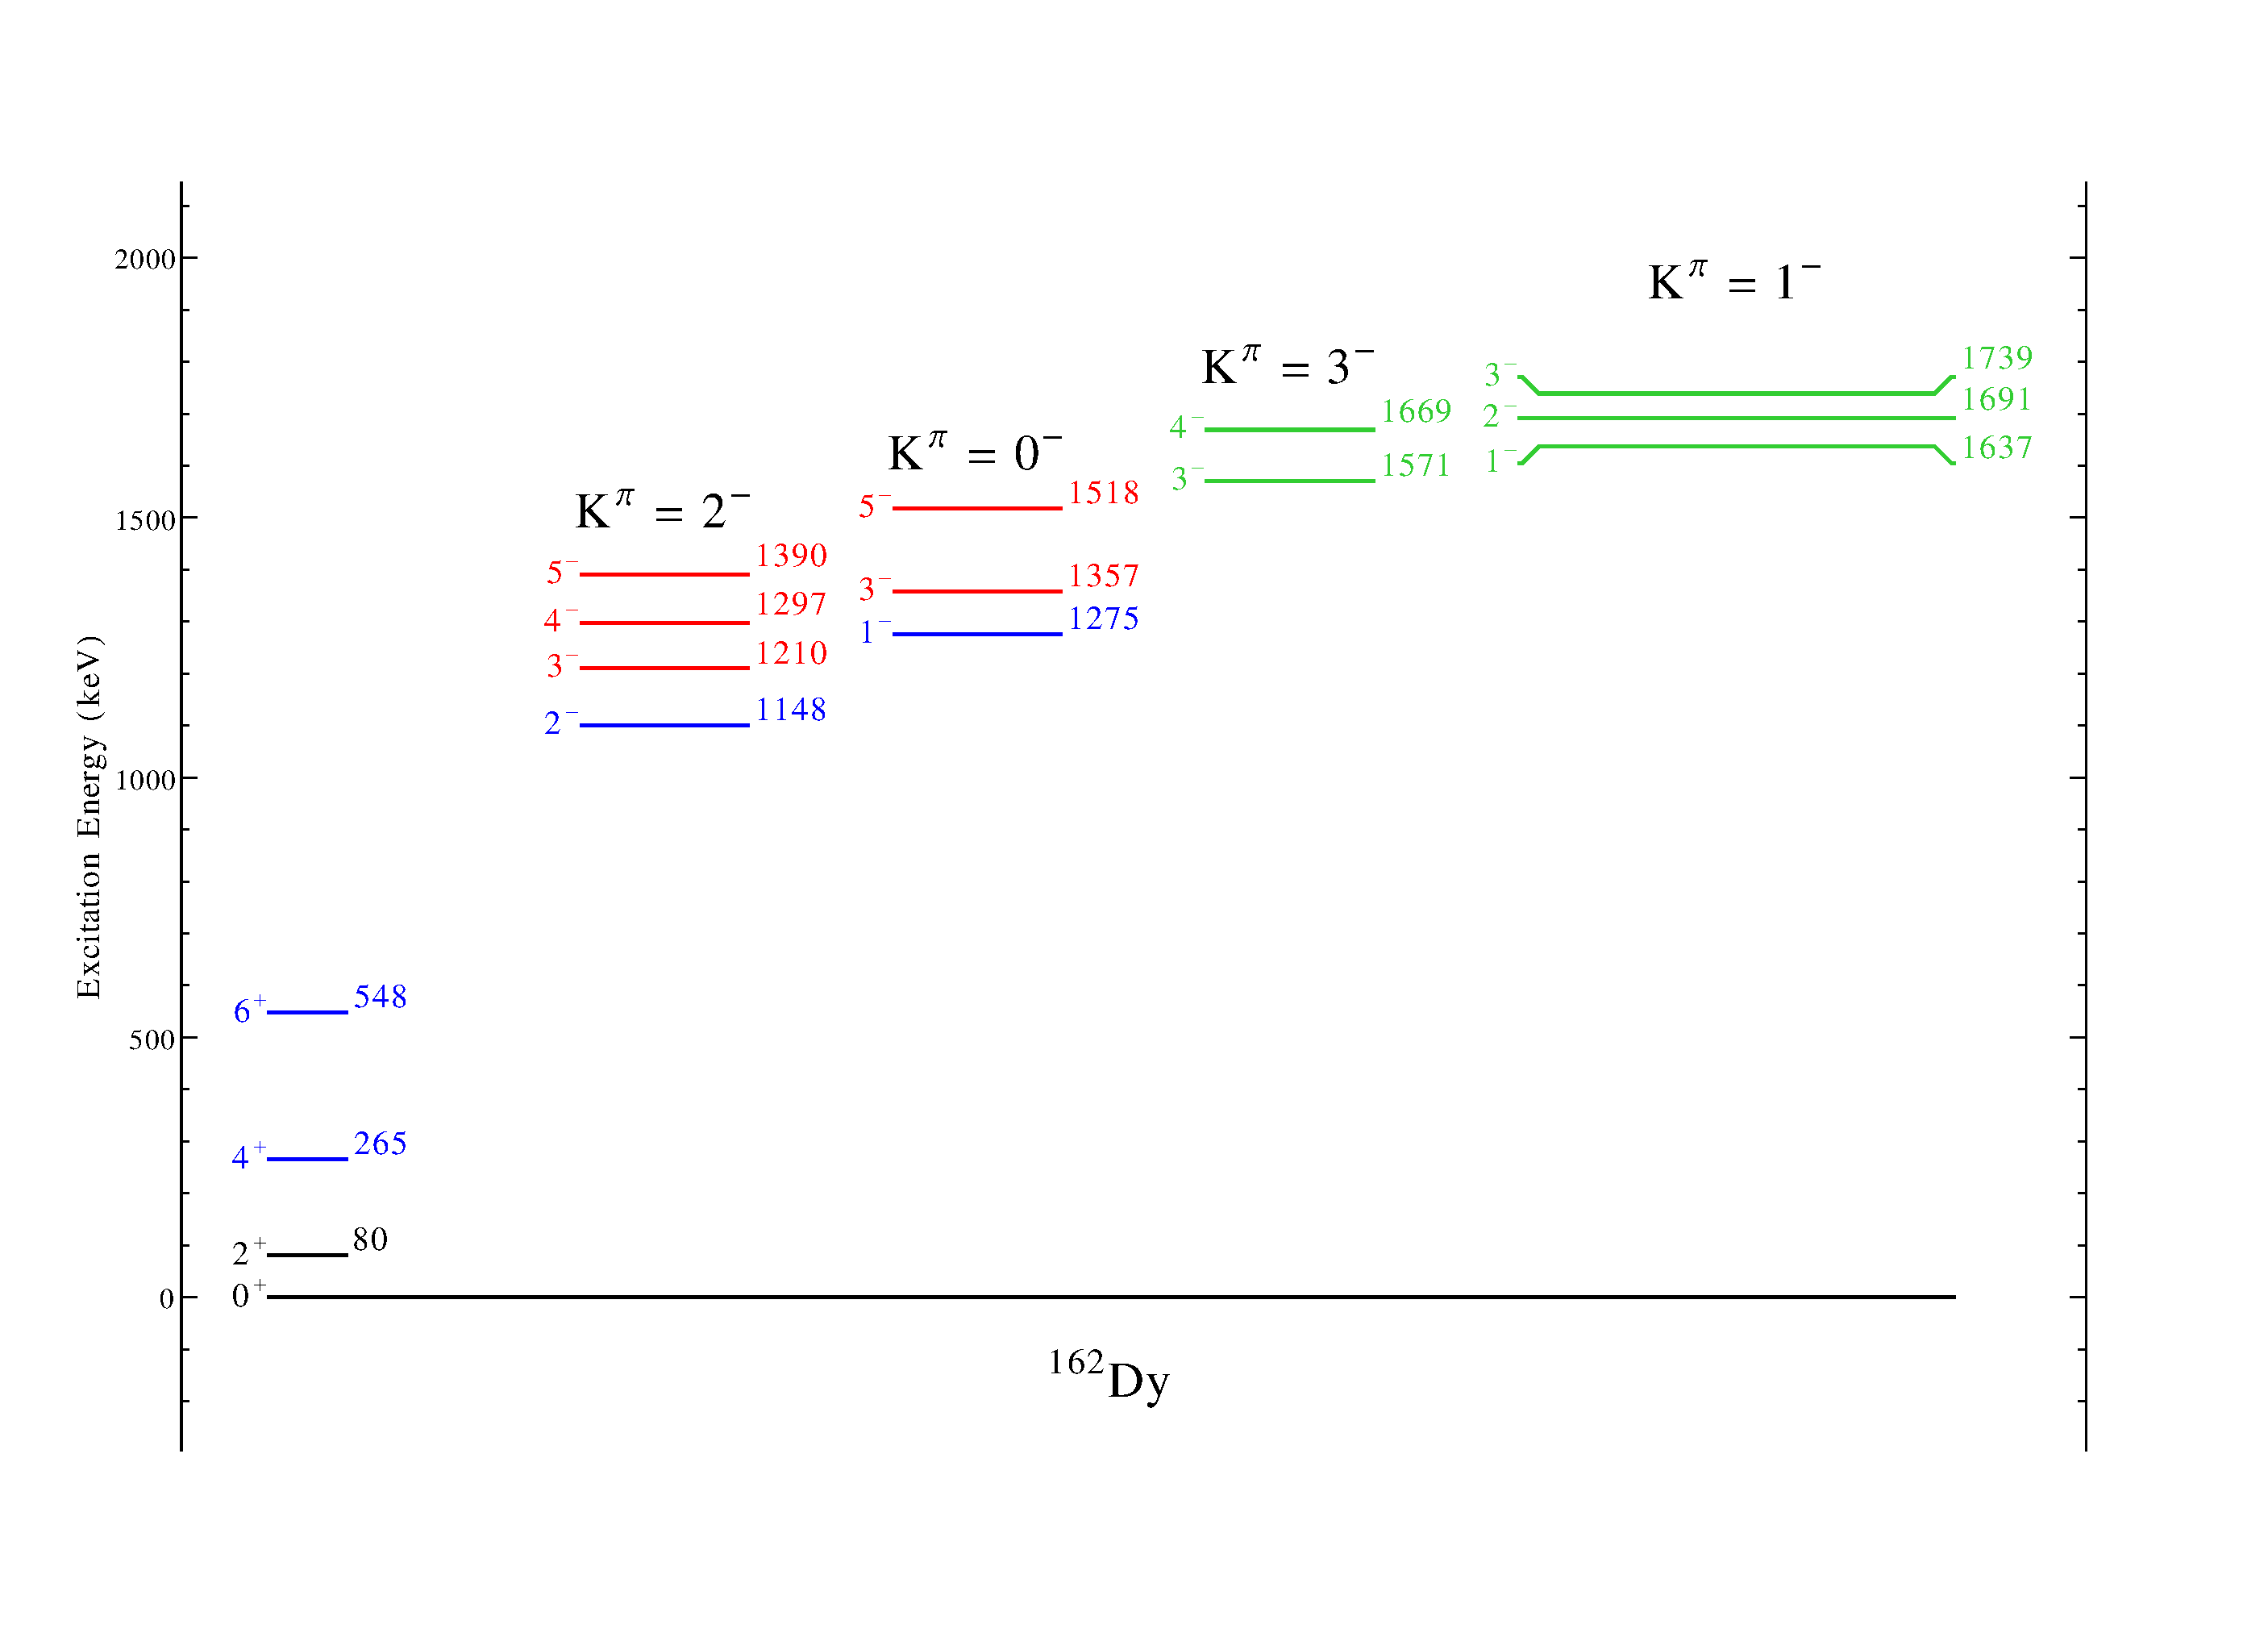
\includegraphics[width=0.95\textwidth]{../Dissertation_Casarella/162Dy_LLoct.pdf}
% \caption{Lowest-lying negative parity bands in $^{162}$Dy with reliable lifetimes measured in our experiments in red, existing literature values in blue, and unreliable lifetimes measured in green (color online). \label{fig:app_162Dy_LLoct}}
% \end{center}
% \end{figure}
% 
% A total of 10 well-convergent level lifetimes were measured (8 of which are new) for three negative parity bands in $^{162}$Dy. All observed transitions from negative parity bands can be seen in Figure \ref{fig:app_162Dy_negparity_202}, with corresponding transition strengths from Table \ref{tab:162Dy_negparity_202}. Absolute intensities of $\gamma$-decays reported in this work can be seen in Table \ref{tab:162Dy_neg202_intensities}. The traditional picture of octupole collectivity in well-deformed nuclei exists with the initial, lowest-lying and fragmented quartet of states of K$^\pi$=0$^-$, 1$^-$, 2$^-$, \& 3$^-$. However, the current ordering of negative parity bands in $^{162}$Dy is difficult (read: impossible) to predict with modern models \cite{Aprahamian200642}. We have measured lifetimes for two bands of this lowest-lying set of states in $^{162}$Dy, where we provide individual discussion on our measurements.
% 
% \begin{table}[h]
% \makebox[\textwidth]{
% \begin{tabular}{llcccllc}
% E$_{level}$ (keV) & E$_\gamma$ (keV) & J$^\pi_{K^\pi_i}$ & J$^\pi_{K^\pi_f}$   & F($\tau$)$_{av}$ & $\tau$ (fs)                     & BR        & B(E1) (mW.u.)\\ \hline \hline
%  1148.20(20) &  260.16(50)               & 2$^-_{2^-_1}$      & 2$^+_{2^+_1}$ &0.074$\pm$0.058& 2100$^{+7200}_{-950}$ $^{[\varsigma]}$          &1.000                 & 8.9$^{+7.3}_{-6.9}$  \\ 
%  1210.05(18) &  247.27(55)$^{[\oslash]}$ & 3$^-_{2^-_1}$      & 3$^+_{2^+_1}$ &0.052$\pm$0.030& 3100$^{+3700}_{-1200}$ $^{[\varsigma]}$         &0.056(2)              & 0.2$^{+0.2}_{-0.1}$ \\
%              &  322.05(51)$^{[\oslash]}$ & 3$^-_{2^-_1}$      & 2$^+_{2^+_1}$ &&                                                            &0.083(2)              & 0.2$^{+0.1}_{-0.1}$ \\
%              &  944.48(50)               & 3$^-_{2^-_1}$      & 4$^+_{0^+_1}$ &&                                                            &0.310(4)              & 0.04$^{+0.03}_{-0.02}$  \\
%              & 1129.46(50)$^{[\oslash]}$ & 3$^-_{2^-_1}$      & 2$^+_{0^+_1}$ &&                                                            &0.552(4)              & 0.04$^{+0.03}_{-0.02}$  \\ 
%  1297.06(27) &  236.09(60)$^{[\oslash]}$ & 4$^-_{2^-_1}$      & 4$^+_{2^+_1}$ &0.103$\pm$0.049& 1400$^{+1500}_{-350}$ $^{[\varsigma]}$          &0.150(5)              & 2.7$^{+0.9}_{-1.4}$    \\
%              &  334.15(50)               & 4$^-_{2^-_1}$      & 3$^+_{2^+_1}$ &&                                                            &0.850(5)              & 5.3$^{+1.8}_{-2.8}$   \\ 
%  1390.52(35) & 1124.88(88)               & 5$^-_{2^-_1}$      & 4$^+_{0^+_1}$ &0.090$\pm$0.082& $>$920 $^{[\varsigma]}$                         &1.000                 & $<$0.3               \\ \hline
%  1275.81(24) & 1195.10(50)               & 1$^-_{0^-_1}$      & 2$^+_{0^+_1}$ &0.568$\pm$0.028& 120$^{+10}_{-10}$ $^{[\vartheta]}$             & 0.605(6)             & 1.0$^{+0.1}_{-0.1}$ \\
%              & 1275.82(53)               & 1$^-_{0^-_1}$      & 0$^+_{0^+_1}$ &&                                                            & 0.395(6)             & 0.5$^{+0.1}_{-0.1}$ \\ 
%  1358.00(30) & 1092.27(71)               & 3$^-_{0^-_1}$      & 4$^+_{0^+_1}$ &0.612$\pm$0.043& 100$^{+20}_{-20}$ $^{[\vartheta]}$             & 0.429(9)             & 1.1$^{+0.3}_{-0.2}$ \\ 
%              & 1277.33(58)               & 3$^-_{0^-_1}$      & 2$^+_{0^+_1}$ &&                                                            & 0.571(9)             & 0.9$^{+0.2}_{-0.2}$  \\ 
%  1518.47(29)&   970.01(55)               & 5$^-_{0^-_1}$ & 6$^+_{0^+_1}$      &0.372$\pm$0.041& 270$^{+80}_{-50}$ $^{[\varsigma]}$              &0.294(7)              & 0.4$^{+0.1}_{-0.1}$         \\
%             &  1252.74(51)               & 5$^-_{0^-_1}$ & 4$^+_{0^+_1}$      &&                                                            &0.706(7)              & 0.4$^{+0.1}_{-0.1}$         \\ \hline
%  1863.85(26)&   900.90(55)               & 2$^-_{2^-_2}$ & 3$^+_{2^+_1}$      &0.297$\pm$0.035& 420$^{+120}_{-80}$ $^{[\varsigma]}$             &0.251(5)              & 0.3$^{+0.1}_{-0.1}$        \\
%             &   975.65(50)               & 2$^-_{2^-_2}$ & 2$^+_{2^+_1}$      &&                                                            &0.749(5)              & 0.6$^{+0.1}_{-0.1}$        \\ 
%  1910.50(26)&   947.51(56)               & 3$^-_{2^-_2}$ & 3$^+_{2^+_1}$      &0.250$\pm$0.063& 550$^{+260}_{-180}$ $^{[\varsigma]}$            &0.552(8)              & 0.4$^{+0.2}_{-0.1}$         \\
%             &  1022.33(53)               & 3$^-_{2^-_2}$ & 2$^+_{2^+_1}$      &&                                                            &0.448(8)              & 0.3$^{+0.1}_{-0.1}$        \\ 
%  1972.99(66)&   912.09(50)               & 4$^-_{2^-_2}$ & 4$^+_{2^+_\gamma}$ &0.205$\pm$0.053& 780$^{+280}_{-210}$    $^{[\varpi]}$       &0.246(13)             & 0.1$^{+0.1}_{-0.1}$\\            
%             &  1010.19(50)               & 4$^-_{2^-_2}$ & 3$^+_{2^+_\gamma}$ &&                                                            &0.754(13)             & 0.3$^{+0.1}_{-0.1}$\\ \hline  
% \end{tabular}
% }\\
% {\small $^{[\oslash]}$: $\gamma$ ray not used in F($\tau$) calculation (F($\tau$)$<$0).}\\
% {\small $^{[\vartheta]}$: F($\tau$) extracted from E$_n$=1.6~MeV angular distributions},
% {\small $^{[\varsigma]}$: F($\tau$) extracted from E$_n$=2.2~MeV angular distributions},
% {\small $^{[\varpi]}$: F($\tau$) extracted from E$_n$=3.1~MeV angular distributions}\\
% {\small $^{[\dagger]}$: Lifetime not reliable (F($\tau$) consistent with zero within 1$\sigma$)}\\
% \caption{Lifetimes of negative parity bands (2$^-$, 0$^-$, 2$^-_2$) in $^{162}$Dy, with experimentally deduced B(E1) in mW.u. \label{tab:app_162Dy_negparity_202}}
% \end{table}
% 
% 
% \subsection{K$^\pi$=2$^-$ Band at 1148~keV}
% %  Assertions from IBM considerations with the inclusion of \textit{p} and \textit{f} bosons imply that the structure of the lowest-lying negative parity bands may not be of purely collective nature  \cite{Aprahamian200642, Iachello_Arima_IBM}.
% 
% % Our measurement of lifetimes in the K$^\pi$=2$^-$ band make a strong case for a two-quasiparticle nature of this band, based on our characteristically weak and noncollective B(E1) transitions to both the $\gamma$-vibrational band and to the ground state. 
% % We start with the K$^\pi$=2$^-$ band. One discrepancy regards our measurement of the bandhead lifetime; the literature lifetime of 303~ps (measured by the delayed coincidence method in \cite{PhysRev.166.1227}) is in stark disagreement with our measured lifetime of 1220~fs. This two order of magnitude difference is alarming and would otherwise spark a mismeasurement of the lifetime, but our placement of the single and most intense $\gamma$ ray at 260~keV in both the excitation function measurements as well as the decently well-behaved energy shift is unambiguous. In addition to our data, it is entirely possible that the wide energy gates used in \cite{PhysRev.166.1227} are seeing a 185~keV $\gamma$ ray from the ground state 4$^+$ member, with a similar lifetime (at 190 ps), which could also explain our discrepancy with literature. 
% We are immediately presented with some of the limitations of DSAM with our measurement of the lifetime of the bandhead of the K$^\pi$=2$^-$ band. Firstly, $\gamma$-ray energies can be heavily attenuated in the physical size of the near-molar-weight target; while we correct for this $\gamma$ absorption in the peak area/intensity, lifetimes from the Doppler shift of $\gamma$-rays sub-500~keV are difficult to extract, as F($\tau$) can be within 1 or 2$\sigma$ of 0. Normally, DSAM measurements are taken at the lowest possible bombarding neutron energy, but due to this attenuation of low-energy $\gamma$ rays, a more precise measurement of the lifetimes in this band are taken from the 2.2~MeV bombarding neutron dataset. While we expect a natural inflation of the lifetimes because of this choice of neutron energy, the vast majority of observed transitions displayed negative (or consistent with zero within 1$\sigma$ uncertainty) F($\tau$) values. This justification is supported by Figure \ref{fig:app_260_DSAM_EXF}, which shows all excitation functions for $\gamma$ rays that both de-excite this band and contribute to the lifetime; take note that the gain in statistics by a factor of $\sim$2 by increasing the neutron energy, where we are exempt from higher-lying decays acting as a contaminant (see the trajectories as the neutron energy increases to 3.1~MeV). Extraction of the lifetime for the bandhead at 2100$^{+7200}_{-950}$~fs involves the measurement of a 260~keV $\gamma$ ray, shown in Figure \ref{fig:app_260_DSAM_EXF}, and does not agree with the literature value of 303~ps \cite{PhysRev.166.1227}, as the shallow F($\tau$) is just over 1$\sigma$ away from 0, making this lifetime partially unreliable. We do not observe the other decay channel to the 3$^+$ member of the $\gamma$-band, as that decay energy is 185~keV, directly on top of our strongest line in our spectra, the ground state 4$^+\rightarrow$2$^+$ transition. With no higher energy decays observed to the ground state, we report this measurement of the bandhead's lifetime, but it should be taken as a tentative, cautious measurement, given the very large discrepancy from literature. However, we regain good lifetime resolution on the measurement of the 3$^-$ and 4$^-$ bandmembers; the former state's lifetime of 3100$^{+3700}_{-1200}$~fs comes from the 944~keV $\gamma$ ray, where the other exit channels have either a negative F($\tau$) value. 
% % Furthermore, \cite{Wu_2minus_2001} outlines the collective intrinsic E1 matrix elements between the 2$^-$ and 2$^+$ band, quoting a value of 0.0053~eb$^{1/2}$ (15.76~mW.u.), and our absolute B(E1) limit is consistent with this value, giving us confidence in a reliable lifetime measurement. 
% 
% Modestly collective transitions to the known $\gamma$-vibrational states are observed leaving the 2$^-$ band at 1148~keV. This highly-favored trend of $\gamma$-rays to the K$^\pi$=2$^+$ band is difficult to ignore in the face of notably strong ($\sim$2-5~mWu), absolute B(E1) measurements between these two modes of excitations. Pascu \cite{Pascu_octupole_2015} stresses the importance of this preferential K$^\pi$=2$^-\rightarrow$K$^\pi$=2$^+$ decay in nearby nuclei via the measurement of direct E3 radiation as a potential octupole-quadrupole coupling, however, this decay pattern could be a product of K-forbidedness, as any decays to the ground state involve $\Delta$K=2 versus the $\Delta$K=0 transitions to the $\gamma$-band. We also mirror these same concerns on the continued study of interband decay radiation in the rare-earth region to fully understand this band; B(E3;5$^-\leftrightarrow$2$^+_\gamma$) strengths would be remarkably useful in this aspect. $^{162}$Dy offers some distinct challenges in terms of the detection of radiation for low-lying excitations; for example, measurement of the interband 2$^-\rightarrow$3$^+_\gamma$ transition lies at 185~keV, placing it directly on top of our most strongly populated 4$^+_{g.s.}\rightarrow$2$^+_{g.s.}$ transition. This experimental challenge is out of the scope of the $\gamma$-singles-based experiments performed in this work at UKAL, and would require much more discriminating coincidence measurements to observe the $\gamma$-decays.
% 
% \begin{figure}[h]
% \begin{center}
% 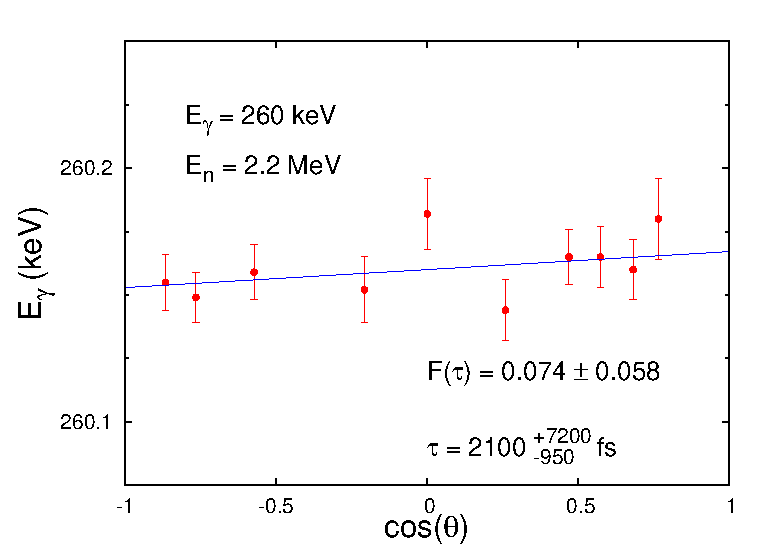
\includegraphics[width=0.49\textwidth]{../Dissertation_Casarella/260_DSAM.eps}
% 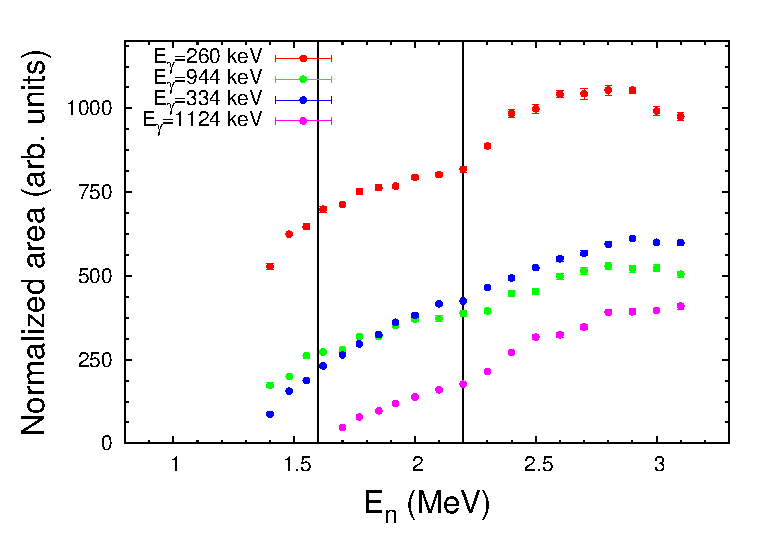
\includegraphics[width=0.49\textwidth]{../Dissertation_Casarella/260_ExF.eps}
% \caption{E$_\gamma$=260~keV $\gamma$ ray (from the E$_{\rm x}$=1148~keV level) Doppler shift and excitation functions for decays from the first 2$^-$ band (color online). \label{fig:app_260_DSAM_EXF}}
% \end{center}
% \end{figure}
% 
% \subsection{K$^\pi$=0$^-$ Band at 1275~keV}
% We have measured lifetimes for the 3 lowest-lying members of the 0$^-$ band, currently assigned as the single octupole vibration in $^{162}$Dy from the clearly collective literature B(E3;3$^-\rightarrow$0$^+_{gs}$) measurements ranging from 1.4-4.7~W.u. \cite{KORTEN_1993,OEHLBERG_BE3}. The deduced lifetime from the direct B(E1)$\uparrow$ measurement in \cite{Zilges_K0dipole} of the bandhead of the K$^\pi$=0$^-$ band has been called into question by the NDS evaluator, with the distinct comment that the $\gamma$-branches of E1 radiation depopulating the state differs drastically from the adopted values. We are confident in our lifetime measurement from the extremely well-defined Doppler energy-shifts of the two de-excitations from this E$_{\rm x}$=1275~keV level (shown in Figure \ref{fig:app_1275_DSAM_EXF}). The 5$^-$ state at 1518~keV is below the threshold to be populated by E$_n$=1.6~MeV neutrons, the de-excitations are not observed until the E$_n$=2.2~MeV dataset; this implies that the resulting lifetime will be inflated, as F($\tau$) is directly related to the bombarding neutron energy.
% 
% Overall in the K$^\pi$=0$^-$ band, we observe inflated, clearly collective B(E1) transition probabilites to the ground state (Table \ref{tab:162Dy_negparity_202}), with excellent agreement to Alaga predictions (Table \ref{tab:162Dy_negparity_ALAGA}). Although these B(E1)s are weaker overall than other confirmed single-phonon octupole vibrations in the region ($^{168}$Er \cite{MCGOWAN_168Er_E3}), the transition probabilities are well above the threshold for what is considered generally non-collective in the mass region ($\sim$10$^{-5}$ mWu strengths). Furthermore, our measured B(E1;1$^-_{K^\pi=0^-}\rightarrow$0$^+_{g.s}$) of 0.002e$^2$fm$^2$ compares very nicely with the systematic behavior of E1 strengths leaving the bandhead of K$^\pi$=0$^-$ bands in deformed rare-earth nuclei (B(E1)$\sim$0.002-0.004~e$^2$fm$^2$) \cite{Borner_collective1999}. From these measured collective E1 strengths, this suggests some significant reflection asymmetry in this K$^\pi$=0$^-$ band, which is especially and notably consistent with the picture of well-behaved octupole collectivity. 
% 
% \begin{figure}[h]
% \begin{center}
% 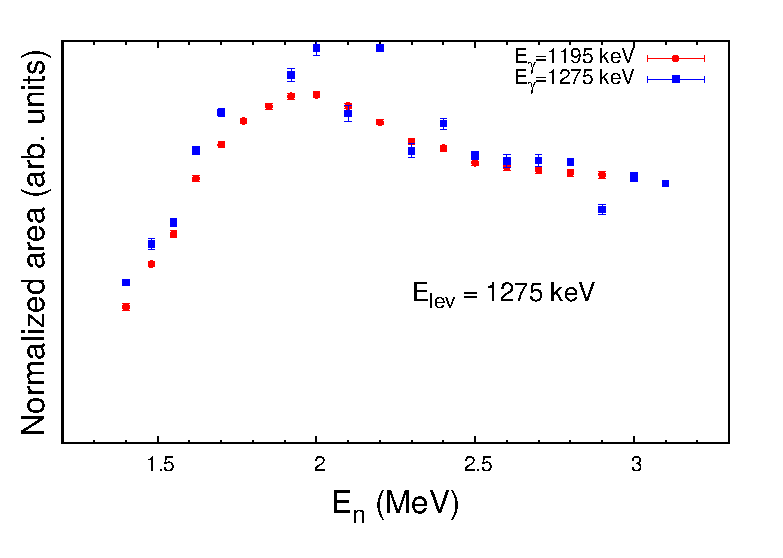
\includegraphics[width=0.75\textwidth]{../Dissertation_Casarella/1195_ExF.eps}\\
% 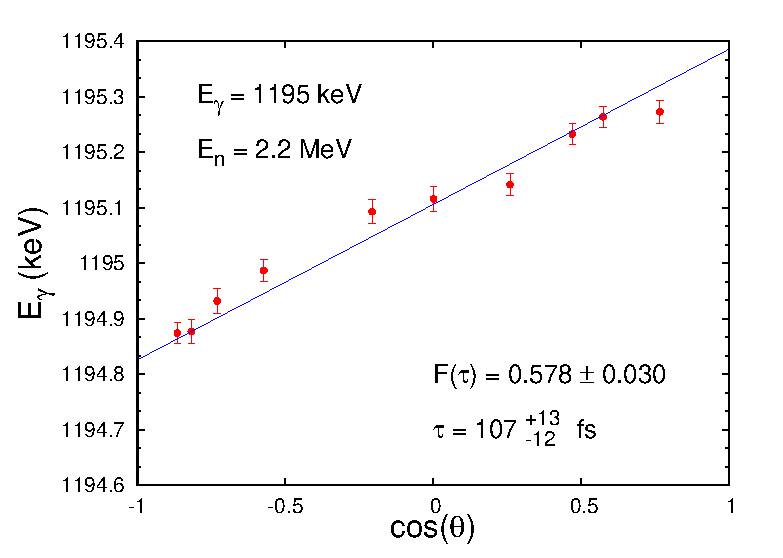
\includegraphics[width=0.49\textwidth]{../Dissertation_Casarella/1195_DSAM.eps}
% 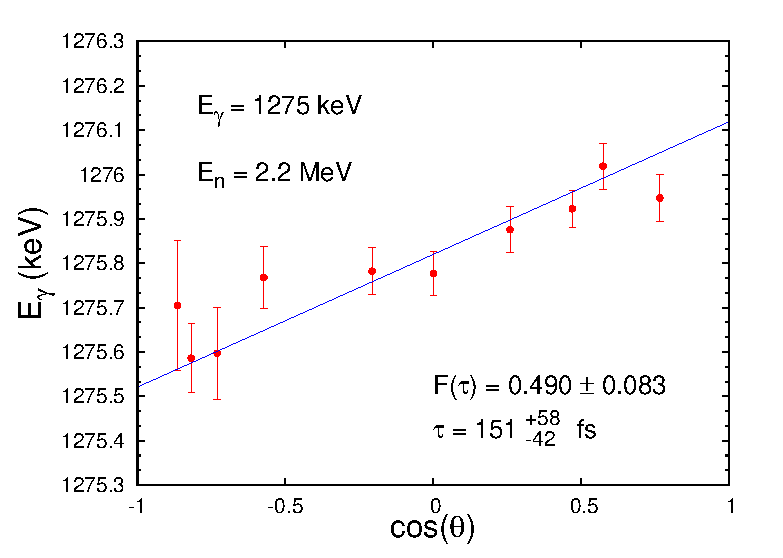
\includegraphics[width=0.49\textwidth]{../Dissertation_Casarella/1275_DSAM.eps}
% 
% \caption{E$_\gamma$=1195 \& 1275~keV (de-excitations from the E$_{\rm x}$=1275~keV level) Doppler shifts and excitation functions (color online). The excitation function (in blue) for the 1275~keV $\gamma$ ray is scaled by a factor of 1.53. \label{fig:app_1275_DSAM_EXF}}
% \end{center}
% \end{figure}
% 
% \begin{figure}[h]
% \begin{center}
% 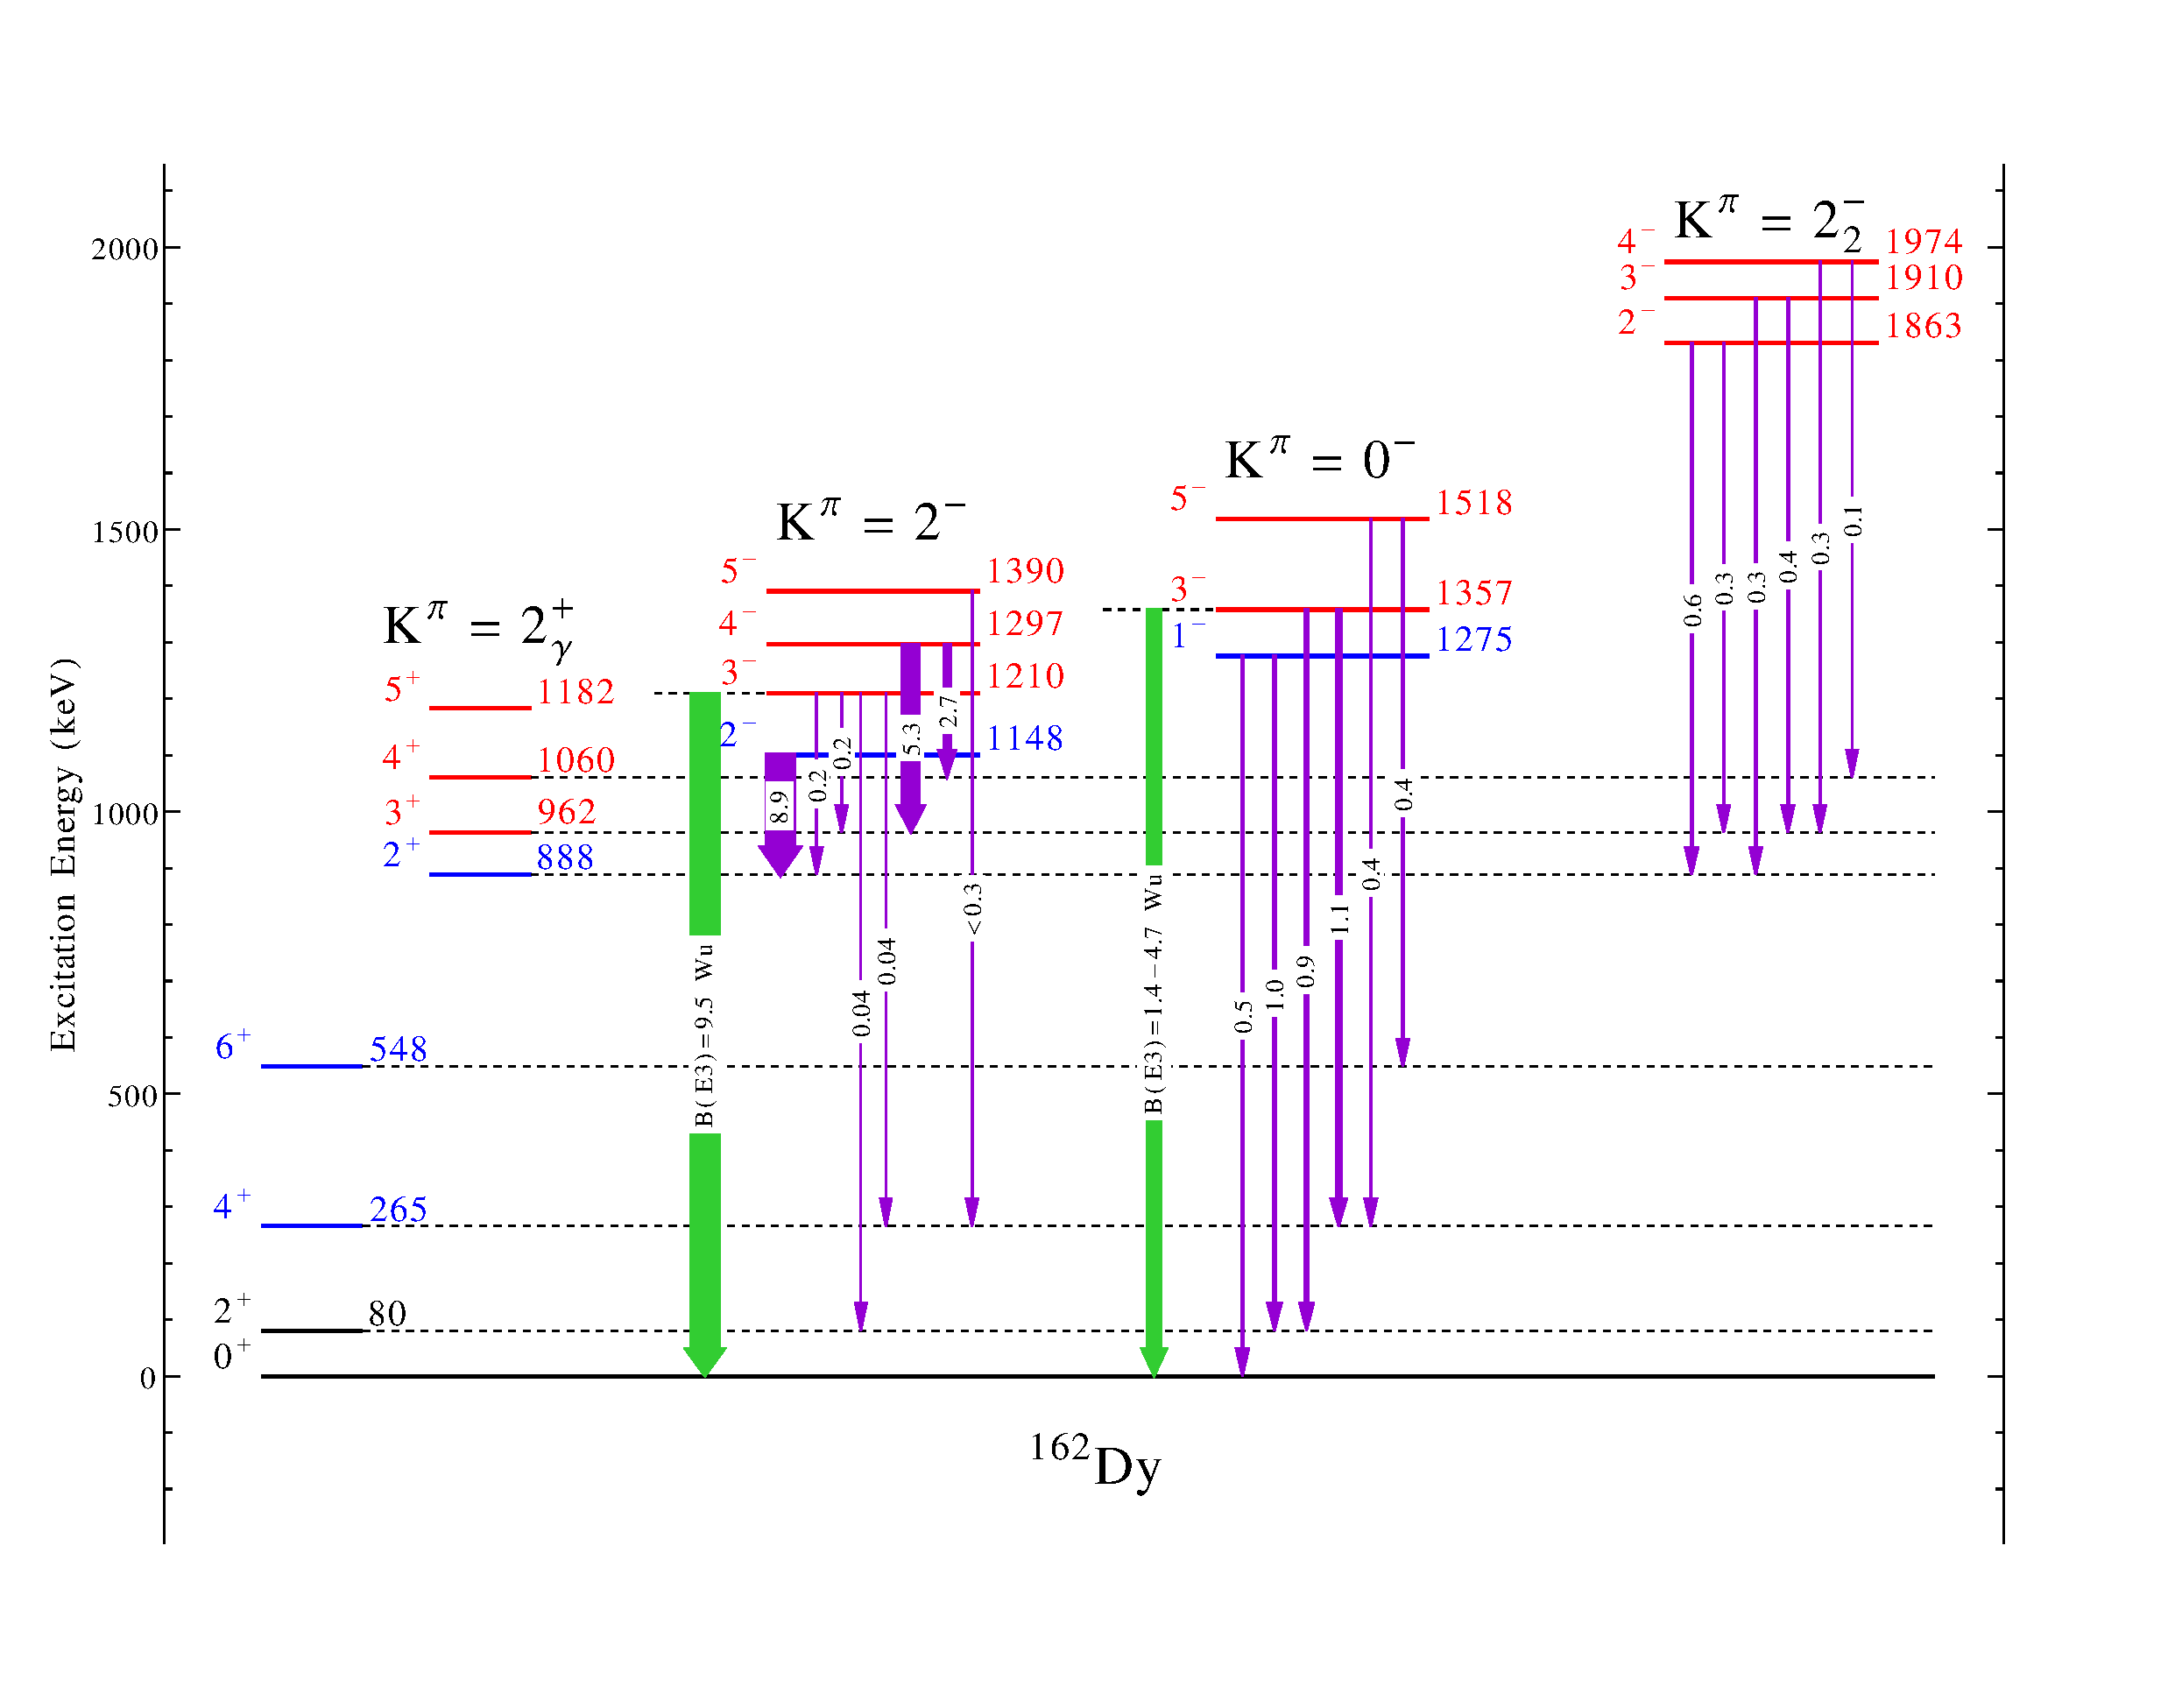
\includegraphics[width=0.98\textwidth]{../Dissertation_Casarella/162Dy_negparity_202.pdf}
% \caption{Observed $\gamma$-decays from negative parity, K$^\pi$=2$^-$, 0$^-$, 2$^-_2$ bands in $^{162}$Dy. Transition strengths are drawn proportional in width to their deduced B(E1), with E1 transitions (B(E1) in milli-Weksskopf units) in violet (color online). \label{fig:app_162Dy_negparity_202}}
% \end{center}
% \end{figure}
% 
% \subsection{K$^\pi$=2$^-_2$ Band at 1863~keV}
% The final set of lifetime measurements of negative parity states is the second K$^\pi$=2$^-$ band. Two $\gamma$-ray placements from \cite{Aprahamian200642} are made into the bandhead of this 2$^-$ band, the 900 and 975~keV transitions, both showing a well-behaved Doppler shift to yield a level lifetime of 420$^{+120}_{-80}$~fs.  We have also placed two $\gamma$-ray transitions from the E$_{\rm x}$=1974~keV 4$^-$ state \cite{BERZINS1995413}, a 912~kev and a 1010~keV decay to the $\gamma$-vibrational band. Confirmation of the placement of these de-excitations is made with the measurement of the excitation functions, shown in Figure \ref{fig:app_1974_DSAM_EXF}; these $\gamma$-rays were also observed in \cite{Aprahamian200642}, but were unplaced in their level scheme. Our absolute intensities are in reasonable agreement with the literature values in \cite{Aprahamian200642,BERZINS1995413}, further justifying their correct placement in the level scheme. 
% 
% \begin{figure}[h]
% \begin{center}
% 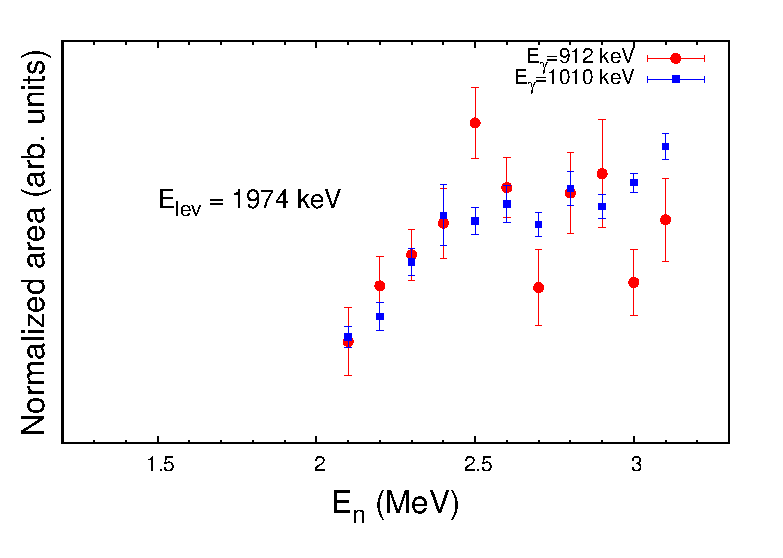
\includegraphics[width=0.75\textwidth]{../Dissertation_Casarella/1974_ExF.eps}\\
% 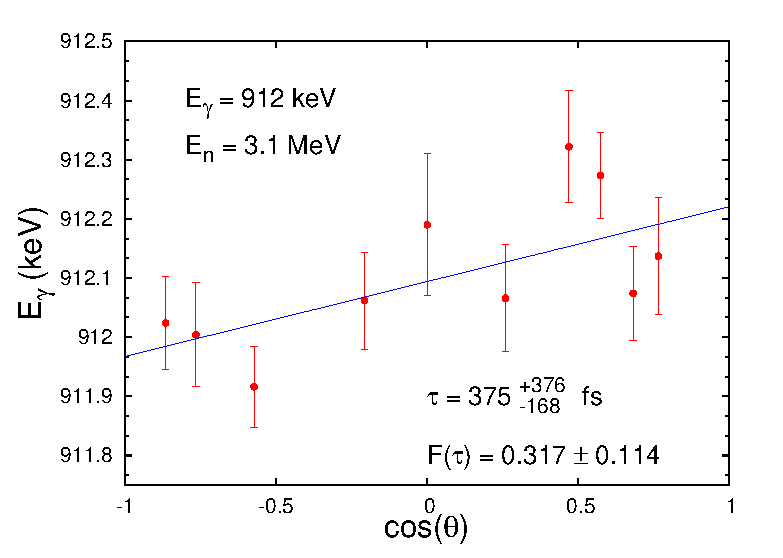
\includegraphics[width=0.49\textwidth]{../Dissertation_Casarella/912_DSAM.eps}
% 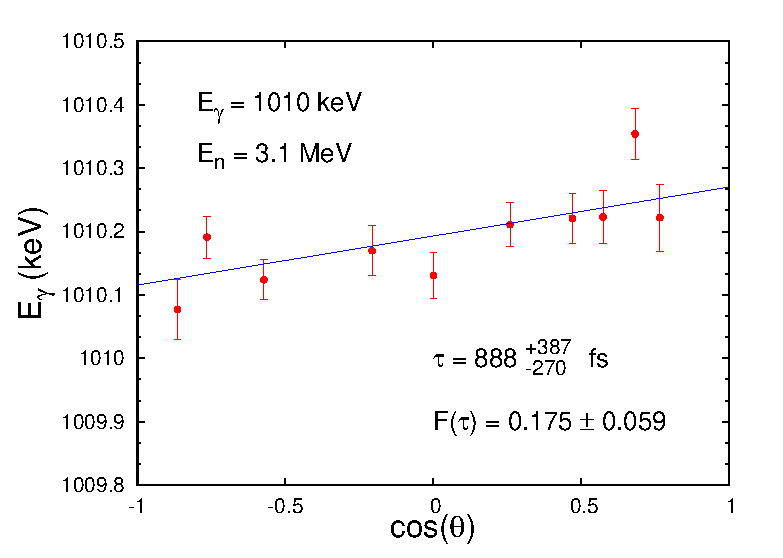
\includegraphics[width=0.49\textwidth]{../Dissertation_Casarella/1010_DSAM.eps}
% 
% \caption{E$_\gamma$=912 \& 1010~keV (de-excitations from the E$_{\rm x}$=1974~keV level) Doppler shifts and excitation functions (color online). The excitation function (in blue) for the 1010~keV $\gamma$ ray is scaled by a factor of 0.33. \label{fig:app_1974_DSAM_EXF}}
% \end{center}
% \end{figure}
% 
% Much like the lower 2$^-$ band, our measurement of mildly inflated B(E1) transition probabilities to the $\gamma$-band is striking, and supports the arguments in numerous works of new, emerging decay patterns \cite{Pascu_octupole_2015,Chakraborty_negparity2012,Spiecker_E1strength} of enhanced E1 transitions to the 2$^+$ band as a differing form of collective dipole excitation built on top of the $\gamma$-vibration. Along the same lines, assertions from IBM considerations with the inclusion of \textit{p} and \textit{f} bosons imply that the structure of the lowest-lying negative parity bands \textit{may not} be of purely collective nature  \cite{Aprahamian200642, Iachello_Arima_IBM}, which supports our experimental findings. Deduced B(E1)s behave well when compared to Alaga considerations (Table \ref{tab:162Dy_negparity_ALAGA}), giving us confidence of correct lifetime measurements. Of particular note, however, is the lower relative B(E1) strength than its lower-energy cousins in the first 2$^-$ band, however, the decays from this band are still above the threshold for what would be considered non-collective. Once again, the interband B(E3) strengths to/from these negative parity bands would be invaluable in the further discussion and feasability of this pattern.
% 
% 
% \begin{table}
% \begin{tabular}{l c c|c}
% K$^\pi$ & $\frac{J_{K_i}\rightarrow J^\prime_{K_f}}{J_{K_i}\rightarrow J^{\prime\prime}_{K_f}}$ & Exp & Th \\
% \hline
% \hline
% \underline{K$^\pi_i$=2$^-$:}   & $\frac{3^-\rightarrow3^+_\gamma}{3^-\rightarrow2^+_\gamma}$ & 1.0 & 1.4 \\
%                                & $\frac{4^-\rightarrow4^+}{4^-\rightarrow3^+}$ & 0.5 & 0.6 \\ \hline
% \underline{K$^\pi_i$=0$^-$:}   & $\frac{1^-\rightarrow2^+}{1^-\rightarrow0^+}$ & 2.0 & 2.0 \\
%                                & $\frac{3^-\rightarrow4^+}{3^-\rightarrow2^+}$ & 1.2 & 1.3 \\
%                                & $\frac{5^-\rightarrow6^+}{5^-\rightarrow4^+}$ & 1.0 & 1.2 \\  \hline
% \underline{K$^\pi_i$=2$^-_2$:} & $\frac{2^-\rightarrow3^+}{2^-\rightarrow2^+}$ & 0.5 & 0.5 \\
%                                & $\frac{3^-\rightarrow3^+}{3^-\rightarrow2^+}$ & 1.6 & 1.4 \\
%                                & $\frac{4^-\rightarrow4^+}{4^-\rightarrow3^+}$ & 0.3 & 0.6 \\ \hline
% 
% \end{tabular}
% \caption{Comparison of E1 transition probabilities from the K$^\pi$=2$^-$, 0$^-$, \& 2$^-$ bands with the Alaga rules. \label{tab:app_162Dy_negparity_ALAGA}}
% \end{table}
% 
% \begin{table}[h]
% \begin{tabular}{cccc}
% A & E$_{\rm x}$ (keV) & K$^\pi_i$ & B(E3;3$^-\rightarrow$0$^+_{gs}$) (W.u.) \\
% \hline
% \hline
% 160 & 1286.711 & 2$^-$ & 16 \\ %0.171 (10) eb
% 160 & 1398.964 & 1$^-$ & 6.0  \\%0.064 eb 
% 160 & 1643.26  & 0$^-$ & 6.1  \\ \hline%0.065 (10) eb \hline
% 162 & 1210 & 2$^-$ & 9.5 $^{[\dagger]}$\\
% 162 & 1357 & 0$^-$ & 1.4-4.7 $^{[\dagger-\ddagger]}$\\ \hline
% 164 & 1039.3 & 2$^-$ &  7.8 \\%0.088 (6) eb $^{[\dagger]}$
% 
% \end{tabular}
% \caption{Known experimentally determined B(E3) probabilities (in W.u.) from [$\dagger$,$\ddagger$] (\cite{McGowan_BE2_1981,OEHLBERG_BE3}, respectively) in the Dysprosium nuclei. \label{tab:app_E3s_Dy}}
% 
% \end{table}
% 
% \begin{table}[h]
% \begin{tabular}{l|l|l}
% % \begin{tabular}{ccc}
% E$_{lev}$ (keV) & E$_\gamma$ (keV) & I$_{\gamma,abs}$ (n,n$^\prime\gamma$)  \\ \hline\hline
%  1148.20(20) &  260.16(50) & 658.762(7.577)\\  \hline
%  1210.05(18) &  247.27(55) &  38.973(1.420)\\
%              &  322.05(51) &  57.699(1.240)\\
%              &  944.48(50) & 216.160(3.227)\\
%              & 1129.46(50) & 384.769(5.182)\\\hline
%  1297.06(27) &  236.09(60) &  43.374(1.380)\\
%              &  334.15(50) & 245.585(4.666)\\\hline
%  1390.52(35) & 1124.88(88) &  94.848(2.193)\\\hline
%  1275.81(24) & 1195.10(50) & 429.944(4.249)\\
%              & 1275.82(53) & 280.443(6.356)\\\hline
%  1358.00(30) & 1092.27(71) & 134.371(1.271)\\
%              & 1277.33(58) & 178.995(6.684)\\\hline
%  1518.47(29)&   970.01(55) &  32.453(0.775)\\
%             &  1252.74(51) &  78.039(1.893)\\\hline
%  1863.85(26)&   900.90(55) &  47.527(1.219)\\
%             &   975.65(50) & 141.639(1.587)\\\hline
%  1910.50(26)&   947.51(56) &  48.580(0.955)\\
%             &  1022.33(53) &  39.474(0.978)\\\hline
%  1972.99(66)&   912.09(50) &  82.148(3.125)\\
%             &  1010.19(50) & 251.922(15.219)\\\hline
% \end{tabular}
%  \caption{Absolute intensities for $\gamma$-decays observed in (n,n$^\prime\gamma$) experiments.  \label{tab:app_162Dy_neg202_intensities}}
% 
% \end{table}
% 
% \section{Conclusions}
% While we cannot place definite octupole characteristics to some of the negative parity states in $^{162}$Dy from the observed E1 transitions, we \textit{can} point future experiments in the right direction to fully ascertain any E3 decays among excited states, based on our measurement of lifetimes and absolute electric dipole reduced transition probabilities. Overall, the story of well-defined, single-phonon octupole correlations in a fragmented quartet of states below the pairing gap in $^{162}$Dy seems indefinite from our incomplete measurement of lifetimes of the negative parity bands. The generally weak, yet still collective B(E1) transition probabilities from the low-lying negative parity bands to the ground state could even imply that octupole correlations are weak in $^{162}$Dy. We have opened a few avenues to study multiphonon effects in regards to octupole-quadrupole coupling in well-deformed nuclei with this data, and hope to see continued study in this area. %Furthermore, we have contributed an exhaustive measurement campaign of the lifetimes of negative parity states under 2.0~MeV in $^{162}$Dy.
% \section{Acknowledgements}
% This work is funded by the National Science Foundation (NSF) under grant numbers PHY-1068192, PHY-1205412, and PHY-0956310. 
% % Special and gracious thanks to S.R.~Lesher, A.~Aprahamian, H.G.~B\"orner, M.~Jentschel, R.F.~Casten, and D.D~Warner for early access to the unpublished GRID lifetime measurements. 
% Special thanks to R. Casten for invaluable physics insight and discussions.